\documentclass[cn,10pt,math=newtx,chinesefont=founder]{../elegantbook}

\title{力學}
\subtitle{2021年}

\author{李宥頡}
\institute{National Taiwan University}
%\date{May 2, 2021}
%\version{4.1}
%\bioinfo{自定义}{信息}


\setcounter{tocdepth}{3}

%\logo{logo-blue.png}
\cover{cover.jpg}

% 本文档命令
\usepackage{array}
\newcommand{\ccr}[1]{\makecell{{\color{#1}\rule{1cm}{1cm}}}}

\definecolor{customcolor}{RGB}{32,178,170}
\colorlet{coverlinecolor}{customcolor}

\begin{document}

\maketitle
\frontmatter

\chapter*{序}
\tableofcontents

\mainmatter

\chapter{運動學}
\section{斜拋}
拋體運動根據運動獨立性(或稱運動重疊原理),可將一曲線運動分為兩個正交方向的直線運動來討論。一般來說,習慣分解成水平方向與鉛直方向,以常見的直角笛卡爾
座標(Cartesian Coordinate),我們將水平方向稱為$x$方向,鉛直方向稱為$y$方向,由於重力恆指向$-y$,故鉛直方向作鉛直上拋運動,且水平方向不受重力,
故水平方向作等速度運動。根據上述,運動的含時參數方程(參數為時間$t$)為
\begin{equation}\label{1.1}
    x = v_0 \cos\theta t\ \ \ \ \ \ \ y = (v_0 \sin\theta)t -\frac{1}{2}gt^2
\end{equation}
\begin{equation}
    v_x = v_0 \cos\theta \ \ \ \ \ \ \ v_y = v_0 \sin\theta - gt
\end{equation}
對於斜拋來說,我們主要對飛行時間$T$、最大高度$H$、水平射程$R$有興趣。直覺上飛行時間應由鉛直方向決定,因為水平方向作等速度運動,看不出時間的影響,故
從鉛直方向的上拋運動判斷。由於上拋上下程的對稱性,飛行時間$T=T_{上}+T_{下}=2T_{上}=\frac{2v_0 \sin\theta}{g}=\frac{2v_{0y}}{g}$。
由於水平方向為等速度運動,水平射程$R = $水平初速 $\times T = \frac{2 v_0 \cos\theta \sin\theta}{g} = \frac{v_0 \sin 2\theta}{g}$。
最後,最大高度$H$由上拋得出,可得$H=\frac{v_0^2 \sin^2\theta}{2g}=\frac{v_{0y}^2}{2g}$。\\
\begin{equation}
\begin{array}{l}
    T = \frac{2v_0 \sin\theta}{g} \\
    R = \frac{v_0 \sin 2\theta}{g} \\
    H = \frac{v_0^2 \sin^2\theta}{2g}
\end{array}
\end{equation}
斜拋重點討論:
\begin{enumerate}
    \item 水平射程$R = \frac{v_0 \sin 2\theta}{g}$在初速$v_0$固定時,
          有一最大值$R_{Max}=\frac{v_0^2}{g}$,
          並發生在$\theta_{Max}=\frac{\pi}{4}$
    \item 同一水平射程$R = \frac{v_0 \sin 2\theta}{g}=\frac{2v_0 \sin \theta \cos \theta}{g}$,
          在固定初速度並透過簡單的代換可知,有兩個拋射角$\theta_1 , \theta_2$滿足同一射程,且
          \begin{equation} \label{1.4}
            \theta_1+\theta_2 = \frac{\pi}{2}
          \end{equation}
\end{enumerate}


\section{斜拋打斜面}
\subsection{運動方程}
在討論斜面上的斜拋運動,我們常選擇平行斜面方向為$x$軸,而垂直斜面方向為$y$軸。分解初速和加速度
之後,此時兩方向的運動均為等加速度運動。\\
\begin{minipage}{\linewidth}
    \begin{minipage}{0.45\linewidth}
\raggedleft
\flushleft
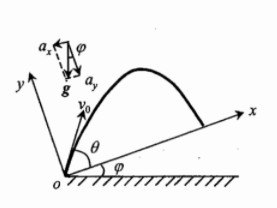
\includegraphics[width=0.5\textwidth]{image/斜拋打斜面.png}
    \end{minipage}
    \hspace{0.05\linewidth}
    \begin{minipage}{0.45\linewidth}
\raggedright
\begin{equation} \label{1.5}
    x = (v_0 \cos\theta t)\pm \frac{1}{2}(g \sin \varphi) t^2 \ \ \ \ \ \ \ y = (v_0 \sin\theta)t -\frac{1}{2}(g\cos \varphi) t^2
\end{equation}
\begin{equation}
    v_x = v_0 \cos\theta \pm (g \sin \varphi) t \ \ \ \ \ \ \ v_y = v_0 \sin\theta - (g\cos \varphi) t
\end{equation}
    \end{minipage}
\end{minipage}
若欲求斜拋打斜面的射程,即令方程式\ref{1.4}中的$y$為0,求出的$x$值即為射程$R$
\begin{equation}
    R = \frac{2v_0^2 \cos (\theta+\varphi)\sin \theta}{g\cos^2 \varphi}
\end{equation}
在固定$v_0$時,最大射程($+$為向上斜拋,$-$為向下斜拋)
\begin{equation}
    R_{Max}=\frac{v_0^2}{g(1\pm \sin \varphi)}
\end{equation}
和相對應的拋射角($-$為向上斜拋,$+$為向下斜拋)
\begin{equation}
    \theta_{Max} = \frac{\pi}{4} \mp \frac{\varphi}{2}
\end{equation}
\begin{proof}
    \\[20em]
\end{proof}

\begin{note}
    如何找三角函數極值:
    \begin{enumerate}
        \item 利用$\sin$,$\cos$的極值分別發生在$\frac{\pi}{2}$,$0$
        \item 利用三角疊合
        \item 利用和差化積、積化和差轉回1.
        \item 一次微分檢驗
    \end{enumerate}
\end{note}




\section{軌跡方程}
雖然運動方程(即位置與時間的函數關係)已經提供充足的解題要素,在實際處理問題上,
軌跡方程因為消去時間參數$t$,因此在解題上面對不含時的問題中,可以更清楚看到初速與
拋射角的關係。將方程 \ref{1.1}代換
\begin{equation}
    t = \frac{x}{v_0 \cos \theta}
\end{equation}
並代入$y$,即可獲得軌跡方程
\begin{equation}
    y=x \operatorname{tan} \theta-\frac{g x^{2}}{2 v_{0}^{2}\cos^2 \theta}
\end{equation}
利用三角恆等式
\begin{equation}
    1+\tan^2 \theta = \sec^2 \theta 
\end{equation}
代換的原因可以使軌跡方程中的角度,變成單一三角函數$\tan \theta$,方便後續討論
\begin{equation} \label{1.7}
    y=x \operatorname{tan} \theta-\frac{g x^{2}}{2 v_{0}^{2}}\left(1+\operatorname{tan}^{2} \theta\right)
\end{equation}
從方程式\ref{1.7}也可以側面證明出斜拋的確是數學上的拋物線$y = ax^2$,且二次項係數為負,代表開口朝下。
求出軌跡方程可幫助我們探討變數$x,y,v_0,\theta$之間的關係。\\
\begin{enumerate}
    \item 

若假定某斜拋的座標起點為原點$(0,0)$,並且在固定初速度$v_0$,並可通過點$(x, y)$,換句話說,方程
\ref{1.7}當中,只剩$\tan \theta$為變數,且可改寫成$\tan \theta$的二次函數
\begin{equation}
    \operatorname{tan}^{2} \theta-\frac{2 v_{0}^{2}}{g x} \operatorname{tan} \theta+\left(\frac{2 v_{0}^{2}}{g x^{2}} y+1\right)=0
\end{equation}
由二次函數的公式解,可求出$\tan \theta$
\begin{equation}
    \operatorname{tan} \theta=\frac{v_{0}^{2}}{g x} \pm \sqrt{\left(\frac{v_{0}^{2}}{g x}\right)^{2}-\left(\frac{2 v_{0}^{2}}{g x^{2}} y+1\right)}
\end{equation}
一般情況下,$\tan \theta$有兩解,且在斜拋的合理拋射角下(銳角),$\tan \theta$和$\theta$為一對一的函數關係,
即同一位置,在固定初速度之下,有兩個拋射角$\theta_1, \theta_2$對應到此位置,並且我們將證明,若此位置在斜面上
(斜角為$\varphi$),兩拋射角之間有關係(對應方程\ref{1.4},即是$\varphi = 0$的情形)
\begin{equation}
    \theta_1+\theta_2 = \frac{\pi}{2}+\varphi
\end{equation}
\begin{proof}
    \\[20em]
\end{proof}
    \item 在初速度和擊中點的$x$座標固定,最大高度$y_{max}$
    \begin{equation}
        y=y_{\max }=\frac{v_{0}^{2}}{2 g}-\frac{g x^{2}}{2 v_{0}^{2}}
    \end{equation}
    且拋射角$\theta_0$必滿足
    \begin{equation}
        \operatorname{tan} \theta=\operatorname{tan} \theta_{0}=\frac{v_{0}^{2}}{g x}
    \end{equation}
    \begin{proof}
        \\[20em]
    \end{proof}

\end{enumerate}
在斜拋打斜面問題中,主要可以分為兩種方法,第一種利用軌跡方程,解代數問題,此方法時常配合二次函數的
解,討論可行的拋射角。第二種方法是利用向量
\begin{equation}
    \vec{r} = \vec{v_0}t+\frac{1}{2}\vec{g}t^2 
\end{equation}
換句話說,位移向量總是$\vec{v_0}t$和$\frac{1}{2}\vec{g}t^2$兩向量做向量加法,
物理意義相當於先利用$v_0$作等速直線運動,再自由落體$\frac{1}{2}gt^2$,搭配斜面
的幾何,即可利用三角函數的正弦定律求解,見例題2-7
\end{document}